\section{Model problema}
U ovom poglavlju formalno se definira problem optimizacije portfelja projektnih aktivnosti. Precizno se opisuju karakteristike aktivnosti, primijenjena ograničenja te jedno-kriterijski i više-kriterijski ciljevi optimizacije koji su korišteni u eksperimentalnoj evaluaciji.

\subsection{Formalna definicija problema}
Problem se definira kao odabir optimalnog podskupa (portfelja) aktivnosti iz većeg, unaprijed definiranog skupa dostupnih aktivnosti.

Neka je $A=\{a_1, a_2, ..., a_n\}$ skup od $n$ dostupnih projektnih aktivnosti. Za svaku aktivnost $a_i \in A$ definirani su sljedeći atributi:
\begin{itemize}
    \item \textbf{Trošak ($c_i$):} Količina budžeta potrebna za izvođenje aktivnosti.
    \item \textbf{Vrijednost ($v_i$):} Povrat na investiciju (ROI) koji se ostvaruje uspješnim završetkom aktivnosti.
    \item \textbf{Nesigurnost trajanja ($T_o, T_m, T_p$):} Trajanje aktivnosti nije deterministička vrijednost, već stohastička varijabla opisana s tri točke procjene: optimističnom, najvjerojatnijom i pesimističnom, koje služe kao parametri za Trokutastu distribuciju u Monte Carlo simulaciji.
\end{itemize}
Cilj je definirati binarni vektor odluke $x=(x_1, x_2, ..., x_n)$, gdje $x_i \in \{0,1\}$. Ako je $x_i=1$, aktivnost $a_i$ je odabrana za uključivanje u portfelj; ako je $x_i=0$, aktivnost se ne izvodi.

\subsection{Ograničenja modela}
Iako realni projekti mogu imati višestruka ograničenja, u ovom modelu implementirano je ključno i najčešće ograničenje u upravljanju portfeljem:
\begin{itemize}
    \item \textbf{Ograničenje budžeta ($B_{max}$):} Ukupni zbroj troškova svih odabranih aktivnosti ne smije prelaziti raspoloživi budžet. Formalno:
    $$ \sum_{i=1}^n c_i x_i \leq B_{max} $$
\end{itemize}
Vrijedi napomenuti da ukupno trajanje portfelja nije tretirano kao strogo ograničenje, već kao izlazna metrika performansi i cilj za minimizaciju. Ovakav pristup je fleksibilniji i realističniji, jer menadžerima često nije cilj samo "uklopiti se" u zadani rok, već pronaći portfelj s najboljim mogućim očekivanim trajanjem za određenu razinu povrata na investiciju.

\subsection{Ciljevi optimizacije}
U skladu s eksperimentalnim dizajnom, definirana su dva različita optimizacijska cilja koja odgovaraju testiranim scenarijima:
\begin{itemize}
    \item \textbf{Jedno-kriterijski cilj: Maksimizacija povrata na investiciju (ROI)}
    Ovaj cilj odgovara klasičnom GA (samo ROI) modelu. Ciljna funkcija je maksimizacija ukupnog zbroja ROI vrijednosti odabranih aktivnosti, uz poštivanje ograničenja budžeta.
    $$ \max \sum_{i=1}^n v_i x_i $$
    \item \textbf{Više-kriterijski cilj: Maksimizacija ROI-a i minimizacija trajanja}
    Ovaj cilj odgovara naprednom hibridnom GA+MC (NSGA-II) modelu i predstavlja srž istraživanja. Ovdje se istovremeno optimiziraju dva, često suprotstavljena, cilja:
    \begin{enumerate}
        \item \textbf{Cilj 1 (Profitabilnost):} Maksimizirati ukupni ROI ($\max \sum v_i x_i$).
        \item \textbf{Cilj 2 (Rizik):} Minimizirati očekivano ukupno trajanje portfelja ($\min E[T(x)]$), gdje je $E[T(x)]$ prosječno trajanje dobiveno Monte Carlo simulacijom za odabrani portfelj $x$.
    \end{enumerate}
\end{itemize}
Ovakav više-kriterijski pristup ne traži jedno jedino "najbolje" rješenje, već skup optimalnih kompromisnih rješenja (Paretov front).

\subsection{Konceptualni model}
Konceptualni model problema, koji prikazuje proces odabira optimalnog portfelja iz skupa dostupnih aktivnosti pod utjecajem ograničenja i optimizacijskih ciljeva, prikazan je na Slici \ref{fig:konceptualni_model}.

\begin{figure}[h!]
    \centering
    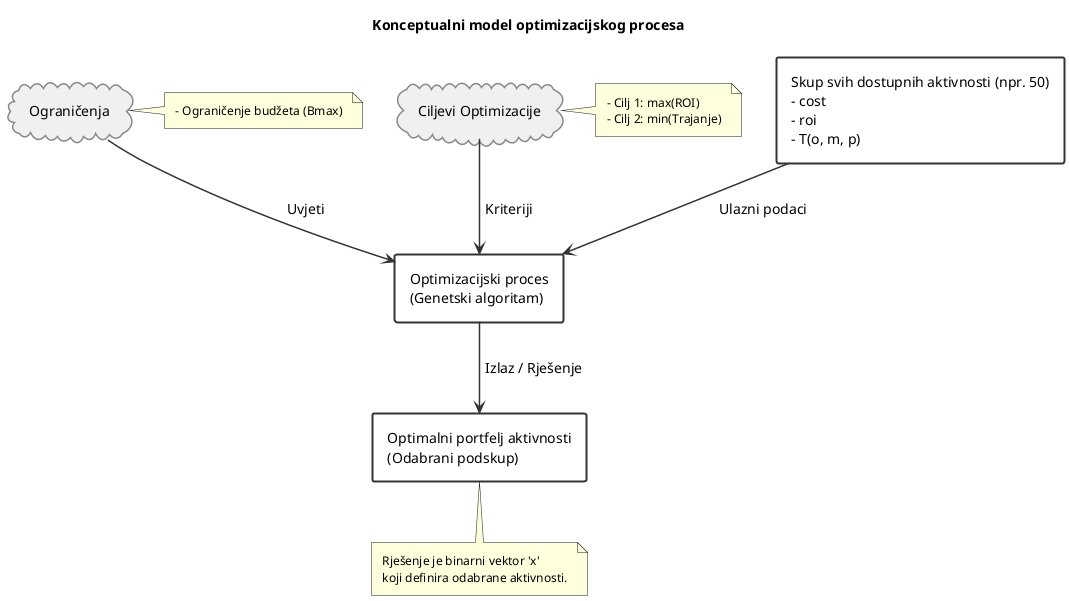
\includegraphics[width=0.9\textwidth]{slike/model_problema.png}
    \caption{Konceptualni model problema optimizacije portfelja projektnih aktivnosti}
    \label{fig:konceptualni_model}
\end{figure}

Ovaj model problema omogućuje jasnu matematičku i vizualnu formalizaciju optimizacijskog zadatka. Precizna definicija ulaza, ograničenja i ciljeva ključna je za primjenu optimizacijskih metoda poput genetskih algoritama u kombinaciji s Monte Carlo simulacijama, kako bi se dobila rješenja visoke kvalitete koja su istovremeno i robusna na prisutne nesigurnosti.
